% !TEX TS-program = XeLaTeX
% !TEX encoding = UTF-8 Unicode

%%%%%%%%%%%%%%%%%%%%%%%%%%%%%%%%%%%%%%%%%%%%%%%%%%%%%%%%%%%%%%%%%%%%%%
%
%	大连理工大学博士论文 XeLaTeX 模版 —— 作者介绍 about.tex
%	版本:0.71
%	最后更新:2010.12.22
%	修改者:Yuri (E-mail: yuri_1985@163.com)
%	编译环境:Ubuntu 10.04 + TeXLive 2010 + TeXworks
%             Windows XP SP3 + CTeXLive 2009 + WinEdt 5.6
%
%%%%%%%%%%%%%%%%%%%%%%%%%%%%%%%%%%%%%%%%%%%%%%%%%%%%%%%%%%%%%%%%%%%%%%

\chapter*{\hfill 作者简介 \hfill}
\addcontentsline{toc}{chapter}{作者简介}
\begin{window}[0,r,{\mbox{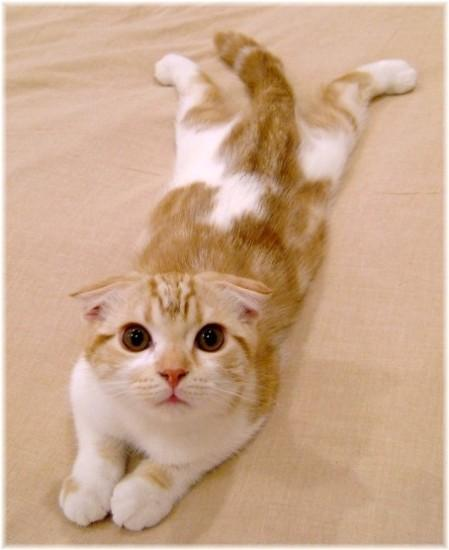
\includegraphics[width=3.5cm]{author.jpg}}},{}]
\end{window}
\daxiaosi
姓名:张 三

性别:男

出生年月:1985~年~00~月~00~日

民族:汉

籍贯:上海市

研究方向:图形图像处理

简历:

\xiaosi
从这里开始写简历

200X.9-200X.7  XX大学XX专业个人简历,从大学起。

200X.9-200X.7  XX大学XX专业个人简历,从大学起。

200X.9-200X.7  XX大学XX专业个人简历,从大学起。

200X.9-200X.7  XX大学XX专业个人简历,从大学起。200X.9-200X.7  XX大学XX专业个人简历,从大学起。200X.9-200X.7  XX大学XX专业个人简历,从大学起。200X.9-200X.7  XX大学XX专业个人简历,从大学起。200X.9-200X.7  XX大学XX专业个人简历,从大学起。
200X.9-200X.7  XX大学XX专业个人简历,从大学起。200X.9-200X.7  XX大学XX专业个人简历,从大学起。200X.9-200X.7  XX大学XX专业个人简历,从大学起。200X.9-200X.7  XX大学XX专业个人简历,从大学起。
